%! Licence = CC BY-NC-SA 4.0

%! Author = mariuszindel
%! Date = 06. Jul 2021
%! Project = DS1-Summary

\section{Blockchain}



\subsection{Bitcoin}

\subsubsection{Introduction}
\begin{itemize}
    \item Experimental digital currency
    \item Fully P2P, no central entity
    \item Maximum of $\sim$ 21 million BTC
    \item Smallest unit: 1 satoshi
    \item Every transaction broadcast to all peers
    \item Validation by proof-of-work (partial hash collision)
    \item Initiator is unknow (Satoshi Nakamoto)
\end{itemize}

\paragraph{Properties}
\begin{itemize}
    \item Not relying on trust, but strong cryptography
    \item Only pseudonimity, no anonymity
    \begin{itemize}
        \item All peers know all transactions
        \item Clustering: if a transaction has multiple input addresses, assume those addresses belong to the same wallet
    \end{itemize}
    \item Not controlled by a single entity
\end{itemize}

\subsubsection{Mechanism}
\paragraph{Wallet}
\begin{itemize}
    \item public-private keys
    \item Public key = bitcoin address (ECDSA 256 bit)
    \item Private key used for signing transactions
\end{itemize}
\paragraph{Transaction}
\begin{itemize}
    \item Peer A wants to send BTC to B, creates transaction message
    \item Transaction contains input / output (src/dst)
    \item Transactions have one or more inputs
    \item Peer A broadcasts the transaction to all peers
    \item Transaction stored in blocks
\end{itemize}
\begin{center}
    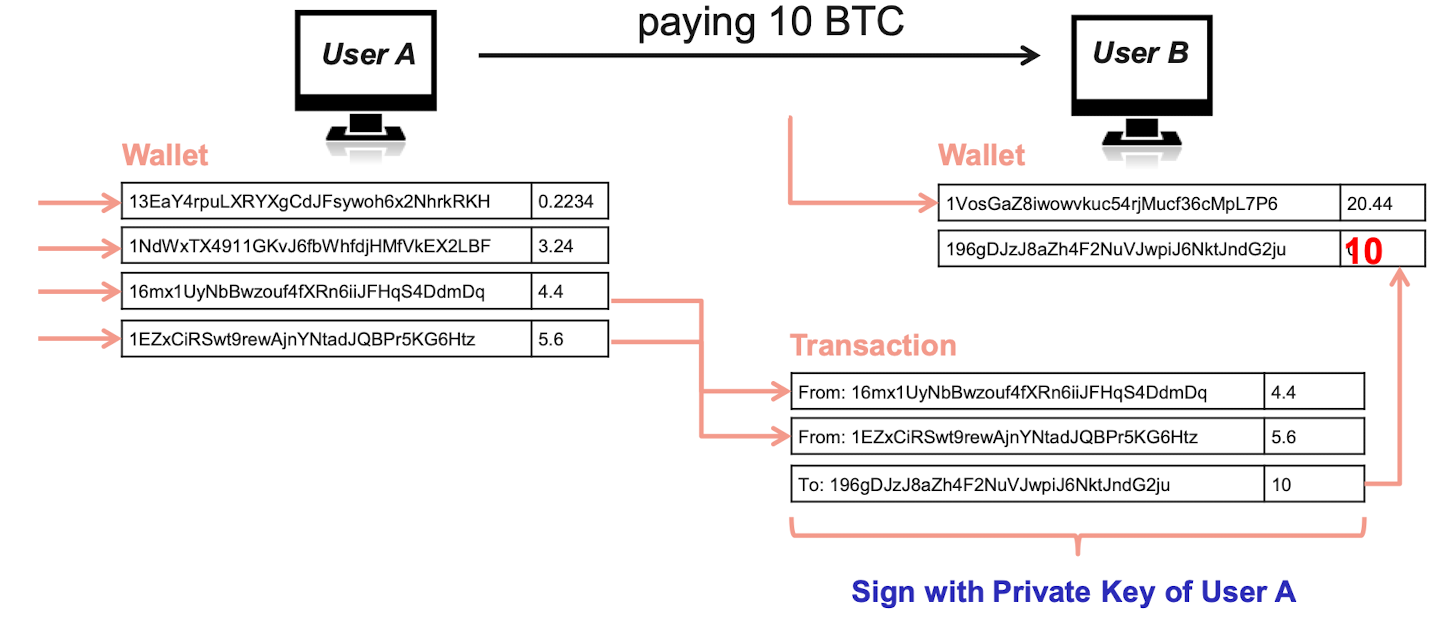
\includegraphics[width=\linewidth]{08-Blockchain/btc-transaction.png}
\end{center}
\vspace{-8pt}
\begin{itemize}
    \item Private Key authorizes the transaction
    \item If keys are stolen, thief is able to use your coins
    \item If keys are lost, coins are lost
    \item In UTXO (unspent transaction output) systems, complete output is spent
\end{itemize}

\paragraph{Blocks}
\begin{itemize}
    \item Block created / verified in $\sim$ 10min
    \item Blocks contain solved crypto puzzles
    \item A Block has a pointer to previous block
    \item Creation of blocks is called mining
\end{itemize}

\paragraph{Mining}
\begin{itemize}
    \item Mining = creating valid blocks
    \item Longest blockchain survive
    \item Dangerous if someone has more than 50\% computing power
\end{itemize}

\subsubsection{Stakeholders}
\begin{center}
    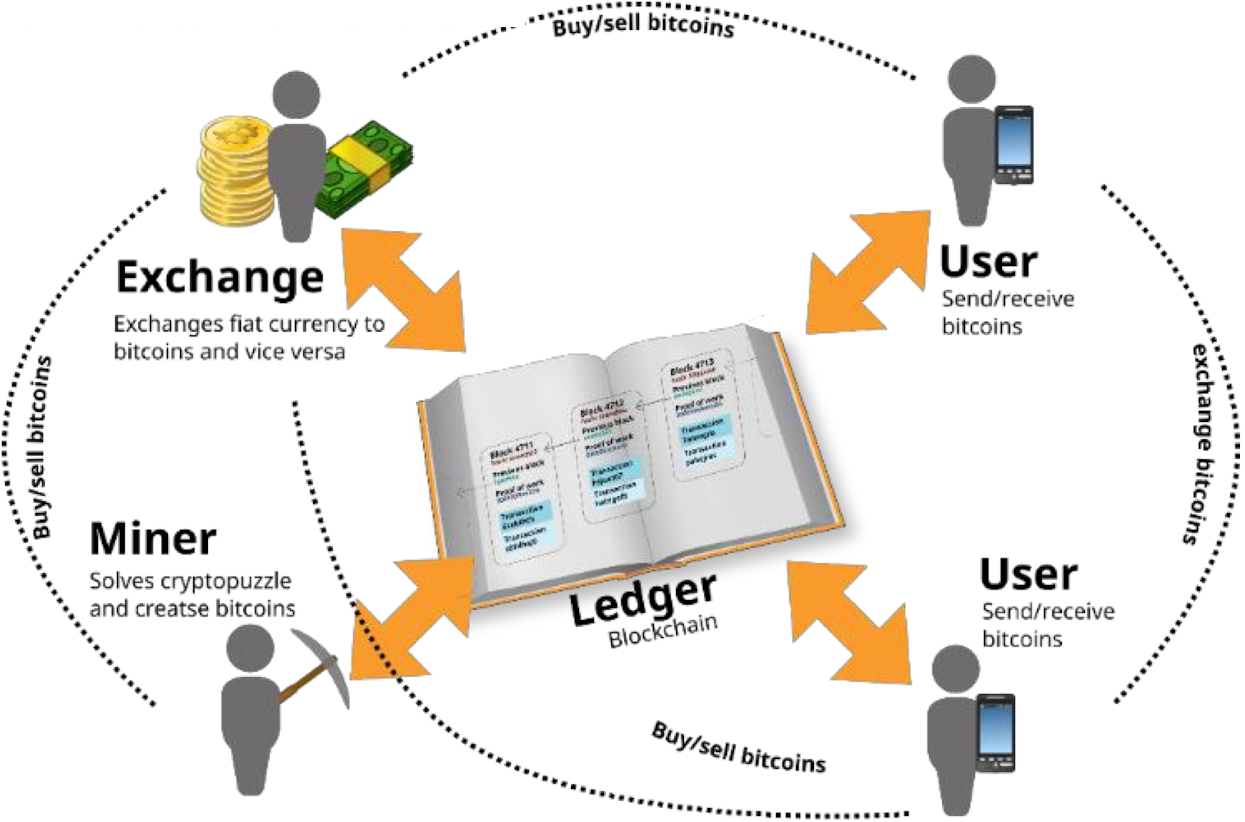
\includegraphics[scale=.25]{08-Blockchain/btc-stakeholders.png}
\end{center}

\subsubsection{51 \% Attack}
If a majority of CPU power is controlled by honest nodes, the honest chain will grow the fastest and outpace any competing chains
\begin{itemize}
    \item \textbf{PoW:} Majority of hashing power
    \item \textbf{PoS:} Majority of coins
    \item Control over 50\% of the scarce resources
\end{itemize}


\subsubsection{Summary}
\begin{itemize}[label={\textcolor{ForestGreen}{+}}]
    \item Low (fixed) tx fees
    \item Scalable (faster HW/Storage)
    \item Anonymity
    \item No major "crashes"
    \item Decentralized
    \item other blockchain use cases $\rightarrow$ Smart contracts
\end{itemize}

\begin{itemize}[label={\textcolor{red}{--}}]
    \item Power consumption as much as Netherlands
    \item Not scalable: 5 transactions per sec
    \item Anonymity can be used for illegal activities
    \item exchange rate fluctuations
\end{itemize}


\subsection{Ethereum}
\subsubsection{Blocktime and gas}
\begin{itemize}
    \item Gas Price set by Miner
    \item Miner decides which transaction at which gas price to include
    \item Gas price too low, longer waiting time until TX will be included
    \item Block time: $\sim$ 14-15s
    \item Smart Contracts are turing complete
    \item Gas price / Gas limit by miners
    \begin{itemize}
        \item If you run out of gas, state is reverted, ETH gone
    \end{itemize}
\end{itemize}

\subsubsection{Smart contract}
\begin{itemize}
    \item For now, proof of work
    \item Every contract is run on every full Ethereum node
    \begin{itemize}
        \item Result on every node is the same
        \item Global computer, always running, always correct
    \end{itemize}
    \item Account-based
    \begin{itemize}
        \item External accounts: controlled by private keys
        \item Contract accounts: never executed on their own
        \begin{itemize}
            \item controlled by code
            \item All action fired from externally controlled accounts
        \end{itemize}
    \end{itemize}
\end{itemize}

\subsubsection{Account vs. UTXO}
\paragraph{Account-based}
\begin{itemize}
    \item Global state stores a list of accounts with balances and code
    \item Transaction is valid if the sending account has enough balance
    \item If the receiving account has code, the code runs, and state may be changed
    \begin{itemize}
        \item Signature must match sending account
    \end{itemize}
    \item Large space savings
    \begin{itemize}
        \item One input - one output - one signature
    \end{itemize}
    \item Simplicity
    \begin{itemize}
        \item Easier to code and understand
        \item Easier for smart contracts (stateful scripting language)
    \end{itemize}
\end{itemize}
\begin{center}
    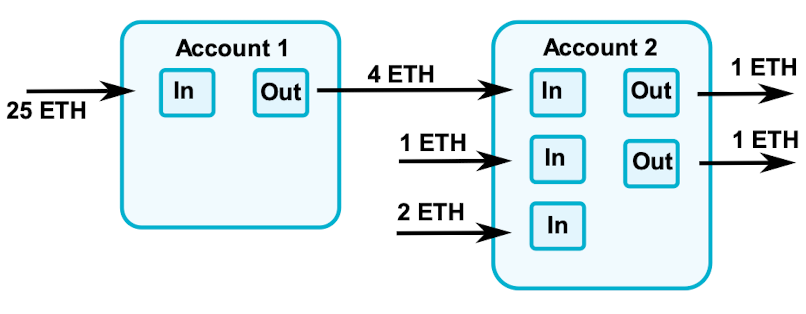
\includegraphics[width=0.6\linewidth]{08-Blockchain/account-based.png}    
\end{center}
\paragraph{UTXO-based}
\begin{itemize}
    \item Every reference input must be valid and not yet spent
    \item Total value of the inputs must equal or exceed the total value of the outputs
    \begin{itemize}
        \item you always spend all outputs
    \end{itemize}
    \item Transaction must have a signature matching the owner of the input for every input
    \begin{itemize}
        \item Script determines if input is valid
    \end{itemize}
    \item Higher degree of privacy
    \begin{itemize}
        \item New address for each TX
        \item No replay attacks - no nonce required
        \item Allows transactions to be processed in parallel
    \end{itemize}
\end{itemize}
\begin{center}    
    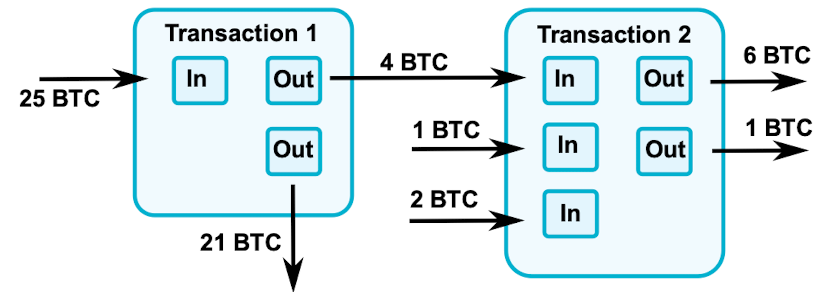
\includegraphics[width=0.6\linewidth]{08-Blockchain/utxo-based.png}
\end{center}

\subsubsection{ERC20}
\begin{itemize}
    \item  ERC20 is a technical standard for smart contracts on the Ethereum blockchain for implementing tokens
\end{itemize}

\subsubsection{Security}
\begin{enumerate}
    \item Reentrancy (Wiedereintritt)
    \item Access Control
    \item Arithmetic Issues
    \item Unchecked Return Values for low level calls
    \item Denial of Service
    \item Bad Randomness
    \item Front Running
    \item Time Manipulation
    \item Short Address Attack
    \item Unknown Unknowns
\end{enumerate}


\subsection{Bitcoin vs. Ethereum}
\paragraph{Bitcoin}
\begin{itemize}
    \item Implementing new features slow
    \item Bitcoin Script limited
    \item Pros and Cons - no silver bullet
\end{itemize}
\paragraph{Ethereum}
\begin{itemize}
    \item Generalized blockchain
    \item Protocols designed from scratch
    \item Mining reward (block every 14s): $\sim$ 2 ETH
\end{itemize}

